% Warehouse Inspector: the project, the pipeline and the platform.
% Build:  tectonic warehouse_inspector_slides.tex      (https://tectonic-typesetting.github.io)
\documentclass[aspectratio=169,10pt]{beamer}

\usepackage[T1]{fontenc}
\usepackage{graphicx}
\usepackage{booktabs}
\usepackage{array}
\usepackage{tikz}
\usetikzlibrary{positioning,arrows.meta,calc,fit,backgrounds}
\usepackage[most]{tcolorbox}
\usepackage{fontawesome}   % v4 icons (fontawesome5 crashes tectonic's XeTeX)
\graphicspath{{figures/}}

% ── colours ────────────────────────────────────────────────────────────────
\definecolor{accent}{RGB}{35,64,190}
\definecolor{ink}{RGB}{20,20,20}
\definecolor{muted}{RGB}{110,110,110}
\definecolor{rulegray}{RGB}{215,215,215}
\definecolor{blueT}{RGB}{31,58,147}   \definecolor{blueBG}{RGB}{237,241,251}  \definecolor{blueLine}{RGB}{120,145,220}
\definecolor{greenT}{RGB}{30,107,52}  \definecolor{greenBG}{RGB}{232,244,235} \definecolor{greenLine}{RGB}{110,175,125}
\definecolor{orangeT}{RGB}{138,75,15} \definecolor{orangeBG}{RGB}{251,242,230}\definecolor{orangeLine}{RGB}{215,160,95}
\definecolor{redT}{RGB}{165,35,35}    \definecolor{redBG}{RGB}{251,236,236}   \definecolor{redLine}{RGB}{215,120,120}
\definecolor{grayT}{RGB}{70,70,70}    \definecolor{grayBG}{RGB}{245,245,245}  \definecolor{grayLine}{RGB}{190,190,190}
\definecolor{belt}{RGB}{59,59,56}     \definecolor{usable}{RGB}{232,232,228}  \definecolor{damaged}{RGB}{208,59,59}

% ── beamer look ────────────────────────────────────────────────────────────
\setbeamertemplate{navigation symbols}{}
\setbeamercolor{normal text}{fg=ink}
\setbeamercolor{structure}{fg=accent}
\setbeamerfont{frametitle}{series=\bfseries,size=\large}
\setbeamertemplate{itemize item}{\color{accent}\tiny$\blacksquare$}
\setbeamertemplate{itemize subitem}{\color{muted}\tiny$\blacktriangleright$}
\setbeamertemplate{enumerate item}{\color{accent}\bfseries\insertenumlabel.}
\setlength{\leftmargini}{1.2em}
\hyphenpenalty=10000 \exhyphenpenalty=10000   % no hyphenated words on slides

\setbeamersize{text margin left=0.9cm, text margin right=0.9cm}
\setbeamertemplate{frametitle}{%
  \vskip 0.7em
  {\usebeamerfont{frametitle}\color{ink}\insertframetitle\par}
  \vskip 0.3em
  
\begin{tikzpicture}
    \fill[rulegray] (0,0) rectangle (\textwidth,0.4pt);
    \fill[accent] (0,-0.9pt) rectangle (1.0cm,1.3pt);
  \end{tikzpicture}\par\vskip 0.1em}

\setbeamertemplate{footline}{%
  \leavevmode\hbox to \paperwidth{\hspace*{0.9cm}\color{muted}\fontsize{7}{8}\selectfont
    Warehouse Inspector --- automated tile inspection\hfill
    \insertframenumber\,/\,\inserttotalframenumber\hspace*{0.9cm}}\vskip 0.3cm}

% ── building blocks ────────────────────────────────────────────────────────
% \panel{blue|green|orange|red|gray}{title}{body}
\newcommand{\panel}[3]{\begin{tcolorbox}[enhanced, colback=#1BG, colframe=#1BG, arc=3pt, boxrule=0pt,
  left=6pt, right=6pt, top=4pt, bottom=5pt, fontupper=\small]%
  {\color{#1T}\bfseries #2}\par\vspace{3pt}#3\end{tcolorbox}}

\tikzset{
  box/.style={draw=#1Line, fill=#1BG, text=#1T, rounded corners=4pt, line width=0.6pt,
              align=center, inner sep=5pt, font=\small\bfseries},
  box/.default=blue,
  sub/.style={font=\tiny\mdseries},
  arr/.style={-{Stealth[length=5pt]}, line width=0.7pt, color=#1},
  arr/.default=muted,
}
\newcommand{\sw}[1]{\tikz[baseline=-0.6ex]\draw[black!40, fill=#1] (0,-0.13) rectangle (0.3,0.13);}
\newcommand{\bignum}[3]{\begin{minipage}[t]{#1}\centering{\fontsize{30}{32}\selectfont\bfseries #2}\\[3pt]{\small\color{muted}#3}\end{minipage}}
\newcommand{\shot}[2]{\tikz\node[inner sep=0pt, draw=rulegray, line width=0.8pt, rounded corners=2pt]{\includegraphics[#1]{#2}};}

\begin{document}

% ════════════════════════════════════════════════════════════════════════════
% Title
% ════════════════════════════════════════════════════════════════════════════
{\setbeamertemplate{footline}{}\setbeamertemplate{background canvas}{\tikz\fill[black] (0,0) rectangle (\paperwidth,\paperheight);}
\begin{frame}[plain]
  \begin{tikzpicture}[remember picture, overlay]
    \node[anchor=west, text=white, font=\fontsize{40}{44}\selectfont\bfseries] at ($(current page.west)+(1.1,1.1)$) {Warehouse Inspector};
    \node[anchor=west, text=white!85!black, font=\Large] at ($(current page.west)+(1.1,-0.05)$) {Automated tile inspection with a {\color{accent!55!white}\bfseries U-Net}};
    \node[anchor=west, text=white!55!black, font=\small] at ($(current page.west)+(1.1,-0.85)$) {From a Colab notebook to the warehouse floor};
    \fill[accent] ($(current page.south west)+(0,1.0)$) rectangle ($(current page.south east)+(0,1.12)$);
    \node[anchor=west, text=white!45!black, font=\scriptsize] at ($(current page.south west)+(1.1,0.45)$) {Project, pipeline \& platform \quad$\bullet$\quad ETH BMAI, week 3};
  \end{tikzpicture}
\end{frame}}

% ════════════════════════════════════════════════════════════════════════════
\begin{frame}{What the Warehouse Inspector is}
  \begin{columns}[T]
    \begin{column}{0.52\textwidth}
      \vspace{0.6em}
      \panel{orange}{The problem}{A recycling warehouse receives reclaimed floor tiles \textbf{by the thousand}.
        Today a person checks every one: is it cracked, chipped, still sellable? It is slow, tiring
        and two inspectors rarely agree on the borderline tiles.}
      \vspace{0.4em}
      \panel{green}{What we built}{An \textbf{inspection station}: each tile rides a conveyor under a camera, a
        \textbf{U-Net} marks the usable surface, and the station decides \textbf{sell or recycle}.
        People only see the tiles the model is unsure about.}
    \end{column}
    \begin{column}{0.40\textwidth}
      \centering
      \begin{tikzpicture}[node distance=0.42cm]
        \node[box=blue, minimum width=3.6cm] (a) {\faCamera\ Photo\\[-1pt]\textnormal{\tiny one tile on the belt}};
        \node[box=orange, minimum width=3.6cm, below=of a] (b) {\faEye\ U-Net\\[-1pt]\textnormal{\tiny belt / usable / damaged, per pixel}};
        \node[box=green, minimum width=3.6cm, below=of b] (c) {\faPercent\ Usable share\\[-1pt]\textnormal{\tiny usable / whole tile}};
        \node[box=gray, minimum width=3.6cm, below=of c] (d) {\faCheckCircle\ Verdict\\[-1pt]\textnormal{\tiny APPROVE if $\geq 85\,\%$, else REJECT}};
        \draw[arr=blueLine] (a) -- (b); \draw[arr=orangeLine] (b) -- (c); \draw[arr=greenLine] (c) -- (d);
      \end{tikzpicture}
    \end{column}
  \end{columns}
\end{frame}

% ════════════════════════════════════════════════════════════════════════════
\begin{frame}{The inspection line}
  \centering
  \vspace{0.3em}
  \shot{width=0.86\textwidth}{inspection_line.png}

  \vspace{0.7em}
  {\small Tiles arrive from intake, the camera and the \textbf{vision model} score each one, and a diverter
  sends it to \textbf{resale} or \textbf{recycling}.\\
  \color{muted}The notebook opens with this animation: it is the machine the students are about to build the brain for.}
\end{frame}

% ════════════════════════════════════════════════════════════════════════════
\begin{frame}{Two halves of the same thing}
  \vspace{0.4em}
  \centering
  \begin{tikzpicture}
    \node[draw=rulegray, rounded corners=5pt, line width=0.7pt, text width=5.6cm, align=center, inner sep=8pt] (ex) {%
      {\bfseries The exercise --- what students build}\\[6pt]
      {\small\color{grayT} A Colab notebook. Students write the dataset, the U-Net, three decision heads,
      run a receptive-field experiment and try transfer learning.}\\[4pt]
      {\small\color{grayT} Live panels grade every step against targets.}\\[8pt]
      \tikz\node[box=blue]{\faLaptop\ \texttt{notebook.ipynb}};};
    \node[draw=rulegray, rounded corners=5pt, line width=0.7pt, text width=5.6cm, align=center, inner sep=8pt, anchor=north west] (pl) at ($(ex.north east)+(1.3cm,0)$) {%
      {\bfseries The platform --- what it becomes}\\[6pt]
      {\small\color{grayT} The same model inside the warehouse's web app: upload photos or use a phone camera,
      review queue, lots, dashboard.}\\[4pt]
      {\small\color{grayT} It runs on the student's own laptop.}\\[8pt]
      \tikz\node[box=green]{\faIndustry\ Inspection platform};};
    \draw[arr=accent] (ex.east) -- (ex.east -| pl.west);
  \end{tikzpicture}

  \vspace{0.7em}
  One file connects them: \textbf{\texttt{platform\_model.pt}}. The notebook exports it in \S 11, the platform loads it
  under \textit{Settings}. What the platform shows is exactly what the student trained.
\end{frame}

% ════════════════════════════════════════════════════════════════════════════
\begin{frame}{The data: one tile per photo}
  \vspace{-0.2em}
  \centering
  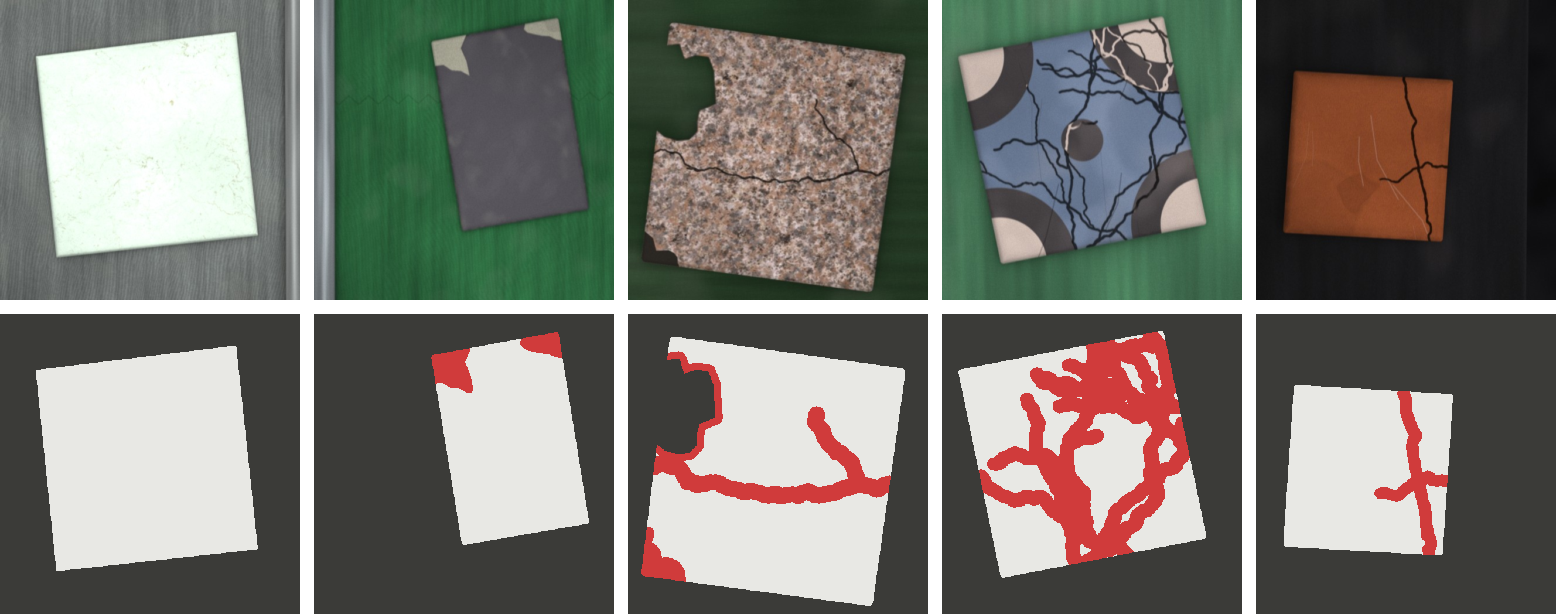
\includegraphics[width=0.74\textwidth]{dataset_strip.png}\\[1pt]
  {\scriptsize\color{muted}\renewcommand{\arraystretch}{1.0}%
  \begin{tabular}{@{}*{5}{>{\centering\arraybackslash}p{0.136\textwidth}}@{}}
    pristine marble & chipped corners & crack + chip & crack network & scratches are fine \\
    {\color{greenT}\bfseries 100\,\% \faCheck} & {\color{greenT}\bfseries 92\,\% \faCheck} & {\color{redT}\bfseries 84.6\,\% \faTimes} & {\color{redT}\bfseries 54\,\% \faTimes} & {\color{greenT}\bfseries 89\,\% \faCheck}
  \end{tabular}}

  \vspace{0.4em}
  \begin{columns}[T]
    \begin{column}{0.30\textwidth}\centering{\fontsize{18}{20}\selectfont\bfseries 5\,000}\\{\footnotesize\color{muted}photos with pixel-exact masks}\end{column}
    \begin{column}{0.30\textwidth}\centering{\fontsize{18}{20}\selectfont\bfseries 55\,\%}\\{\footnotesize\color{muted}approved; 37\,\% are pristine}\end{column}
    \begin{column}{0.34\textwidth}\centering{\fontsize{18}{20}\selectfont\bfseries 6 $\times$ 5}\\{\footnotesize\color{muted}materials $\times$ belts, CC0 textures}\end{column}
  \end{columns}
\end{frame}

% ════════════════════════════════════════════════════════════════════════════
\begin{frame}{Three classes, one rule}
  \begin{columns}[T]
    \begin{column}{0.47\textwidth}
      \vspace{0.2em}
      {\small\bfseries Every pixel is one of three classes}\\[4pt]
      \renewcommand{\arraystretch}{1.25}
      \begin{tabular}{@{}l l p{3.6cm}@{}}
        \toprule
        \sw{belt}    & \textbf{0 belt}    & {\small not part of the tile} \\
        \sw{usable}  & \textbf{1 usable}  & {\small surface that can be sold} \\
        \sw{damaged} & \textbf{2 damaged} & {\small cracks, chips, missing pieces + a 3\,\% cutting margin} \\
        \bottomrule
      \end{tabular}

      \vspace{0.9em}
      \panel{orange}{The hard part}{Stains, dirt and scratches are \textbf{not} damage: the tile can be
      cleaned. A thin crack and a dark vein of marble look alike up close.}
    \end{column}
    \begin{column}{0.47\textwidth}
      \vspace{0.2em}
      \panel{blue}{The decision rule}{%
        \[ \text{usable share} = \frac{\text{usable pixels}}{\text{usable} + \text{damaged pixels}} \]
        \vspace{-4pt}
        \begin{itemize}
          \item $\geq 85\,\%$ $\rightarrow$ \textbf{APPROVE}: sell it, cut down if needed
          \item $< 85\,\%$ $\rightarrow$ \textbf{REJECT}: recycle it
        \end{itemize}
        \vspace{2pt}
        {\scriptsize\color{muted}Measured on the tile, not on the photo: a small tile far from the camera is judged like a big one.}}
      \vspace{0.2em}
      {\footnotesize One number, \texttt{data.USABLE\_THRESHOLD}, used by the notebook and the platform.}
    \end{column}
  \end{columns}
\end{frame}

% ════════════════════════════════════════════════════════════════════════════
\begin{frame}{The pipeline: four ways to reach a verdict}
  \vspace{0.5em}
  \centering
  \begin{tikzpicture}[node distance=0.5cm]
    \node[box=gray] (x) {\faPictureO\ Photo\\[-1pt]\textnormal{\tiny $1\times256\times256$}};
    \node[box=blue, right=of x] (enc) {Encoder\\[-1pt]\textnormal{\tiny conv + pool, $\times$ depth}};
    \node[box=orange, right=of enc] (b) {Bottleneck\\[-1pt]\textnormal{\tiny $C\times H'\times W'$}};
    \node[box=blue, right=of b] (dec) {Decoder\\[-1pt]\textnormal{\tiny up-conv + skips}};
    \node[box=green, right=of dec] (m) {Class map\\[-1pt]\textnormal{\tiny $3\times256\times256$}};
    \draw[arr] (x) -- (enc); \draw[arr] (enc) -- (b); \draw[arr] (b) -- (dec); \draw[arr] (dec) -- (m);
    \draw[arr=blueLine, dashed, rounded corners=6pt] (enc.north) -- ++(0,0.45) -| node[pos=0.25, above, font=\tiny, text=muted]{skip connections} (dec.north);

    \node[box=orange, below=0.95cm of enc, text width=1.55cm] (f) {FNN head\\[-1pt]\textnormal{\tiny pooled vector $\rightarrow$ p(approve)}};
    \node[box=orange, below=0.95cm of b, text width=1.55cm] (c) {CNN head\\[-1pt]\textnormal{\tiny spatial map $\rightarrow$ p(approve)}};
    \node[box=orange, below=0.95cm of dec, text width=1.55cm] (r) {Regressor\\[-1pt]\textnormal{\tiny map $\rightarrow$ usable share}};
    \node[box=green, below=0.95cm of m, text width=1.55cm] (t) {Threshold\\[-1pt]\textnormal{\tiny count pixels, apply 85\,\%}};
    \draw[arr=greenLine] (m) -- (t);
    \draw[arr=orangeLine] (b.south) -- (f.north); \draw[arr=orangeLine] (b) -- (c); \draw[arr=orangeLine] (b.south) -- (r.north);
  \end{tikzpicture}

  \vspace{0.2em}
  \begin{columns}[T]
    \begin{column}{0.45\textwidth}
      \panel{green}{Segment, then count}{The U-Net draws the map; the rule does the rest. Transparent: you can
      \emph{see} why a tile was rejected.}
    \end{column}
    \begin{column}{0.45\textwidth}
      \panel{orange}{Decide from the latent space}{Small heads on the frozen bottleneck. What survives the
      compression, and does throwing away \emph{where} hurt?}
    \end{column}
  \end{columns}
\end{frame}

% ════════════════════════════════════════════════════════════════════════════
\begin{frame}{What students build, step by step}
  \vspace{0.1em}
  \small
  \renewcommand{\arraystretch}{1.12}
  \begin{tabular}{@{}r p{3.0cm} p{5.5cm} p{4.4cm}@{}}
    \toprule
    \textbf{\S} & \textbf{Step} & \textbf{They write} & \textbf{The question it answers} \\
    \midrule
    2   & Dataset            & a \texttt{Dataset}: photo, class map, label \faPencil & can we feed the model correctly? \\
    3   & First U-Net        & \texttt{encode} / \texttt{decode}, the training loop \faPencil & is segment-and-count enough? \\
    4--5& FNN and CNN heads  & two classifiers on the bottleneck \faPencil & does the layout of the damage matter? \\
    6--7& Evaluation         & --- (scoreboard, inspector, game) & which tiles fail, and why? \\
    8   & Receptive field    & --- (depth-2/3/4 experiment) & why cracks look like stains \\
    9   & Challenge          & improved U-Net, heads, a regressor \faPencil & can we beat every target? \\
    10  & Transfer learning  & the decoder of a ResNet-18 U-Net \faPencil & do ImageNet features help? \\
    11  & Deploy             & --- (export + download) & does it work in the product? \\
    \bottomrule
  \end{tabular}

  \vspace{0.4em}
  {\small \faPencil\ = one of the 11 TODO cells.} {\small Every section ends with a \faCompass\ \emph{Why this step?} note that hands its answer to the next.}
\end{frame}

% ════════════════════════════════════════════════════════════════════════════
\begin{frame}{Why the first model fails: the receptive field}
  \begin{columns}[T]
    \begin{column}{0.50\textwidth}
      \vspace{0.6em}
      \panel{blue}{What a pixel can see}{Each output pixel of a CNN depends on a limited patch of the input,
      its \textbf{receptive field}. If the patch is smaller than the pattern, a crack and a dark stain look the same.}
      \vspace{0.4em}
      \panel{green}{The experiment (\S 8)}{Train the same U-Net at \textbf{depth 2, 3 and 4}. Measure the
      theoretical and the \emph{effective} receptive field (input gradients), and click a spot on a tile
      to see what each model sees there.}
    \end{column}
    \begin{column}{0.42\textwidth}
      \vspace{0.8em}
      \centering
      {\small\bfseries Threshold accuracy on the test set}\\[5pt]
      \renewcommand{\arraystretch}{1.25}
      \begin{tabular}{@{}lr@{}}
        \toprule
        Basic U-Net (\S 3) & 86.3\,\% \\
        DepthUNet, depth 2 & 92.4\,\% \\
        DepthUNet, depth 3 & 92.5\,\% \\
        DepthUNet, depth 4 & 92.8\,\% \\
        \bottomrule
      \end{tabular}

      \vspace{0.8em}
      \panel{orange}{The lesson}{Depth sharpens the masks, but the verdict saturates. The rest has to come
      from a better architecture, training and pretrained features.}
    \end{column}
  \end{columns}
\end{frame}

% ════════════════════════════════════════════════════════════════════════════
\begin{frame}{The journey in numbers}
  \vspace{0.5em}
  \centering
  \bignum{0.28\textwidth}{\color{muted}86.3\,\%}{basic U-Net (\S 3)}\hfill
  \bignum{0.28\textwidth}{\color{accent}97.3\,\%}{improved U-Net (\S 9)}\hfill
  \bignum{0.28\textwidth}{\color{greenT}98.5\,\%}{pretrained ResNet-18 (\S 10)}

  \vspace{0.3em}
  {\small\color{muted}threshold-rule accuracy on 750 test tiles}

  \vspace{0.6em}
  \renewcommand{\arraystretch}{1.1}
  \begin{tabular}{@{}lcccc@{}}
    \toprule
    & \textbf{mean IoU} & \textbf{usable-share error} & \textbf{CNN head} & \textbf{regressor} \\
    \midrule
    Basic U-Net     & 0.587 & 7.5 pp  & 70.8\,\% & --- \\
    Improved U-Net  & 0.935 & 1.86 pp & 93.1\,\% & 91.7\,\% \\
    ResNet-18 U-Net & \textbf{0.958} & \textbf{0.92 pp} & --- & \textbf{94.1\,\%} \\
    \midrule
    \color{muted}Target (\S 9) & \color{muted}$\geq$ 0.90 & \color{muted}$\leq$ 2.5 pp & \color{muted}$\geq$ 92\,\% & \color{muted}$\geq$ 90\,\% \\
    \bottomrule
  \end{tabular}
\end{frame}

% ════════════════════════════════════════════════════════════════════════════
\begin{frame}{Same tiles, different models}
  \vspace{0.2em}
  \centering
  \begin{tikzpicture}
    \node[inner sep=0pt] (g) {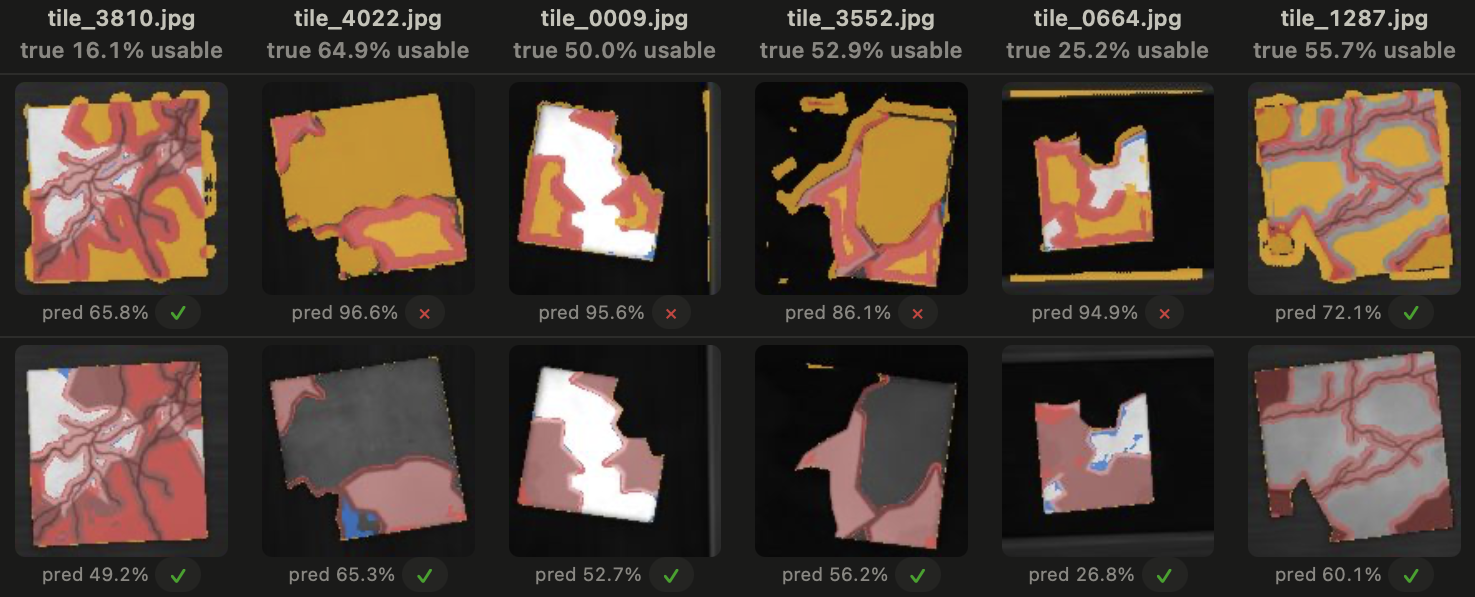
\includegraphics[width=0.78\textwidth]{colab_gallery.png}};
    \node[anchor=east, font=\scriptsize\bfseries, align=right] at ($(g.west)+(-0.1,0.55)$) {Basic\\U-Net\\(\S 3)};
    \node[anchor=east, font=\scriptsize\bfseries, align=right] at ($(g.west)+(-0.1,-1.25)$) {Improved\\U-Net\\(\S 9)};
  \end{tikzpicture}

  \vspace{0.5em}
  {\scriptsize
  \sw{damaged} missed damage \quad
  \sw{damaged!45!black} damage found \quad
  \sw{blue!70} good surface cut away \quad
  \sw{orange} tile / belt confused \quad
  \sw{gray} correct}\\[3pt]
  {\small The six test tiles where the basic model misses the most damage, from a real Colab run.
  The basic U-Net approves four of them; the improved one gets all six right.}
\end{frame}

% ════════════════════════════════════════════════════════════════════════════
\begin{frame}{An interactive notebook}
  \vspace{0.5em}
  \begin{columns}[T]
    \begin{column}{0.31\textwidth}
      {\bfseries\color{blueT}\faLineChart\ Train}\\[3pt]
      \small
      \textbf{Live dashboard}\\{\color{muted}loss and accuracy per epoch, against the target}\\[4pt]
      \textbf{Architecture diagram}\\{\color{muted}every block with its shape}
    \end{column}
    \begin{column}{0.31\textwidth}
      {\bfseries\color{greenT}\faCheckSquareO\ Evaluate}\\[3pt]
      \small
      \textbf{Scoreboard}\\{\color{muted}every method against its target, all attempts kept}\\[4pt]
      \textbf{Confusion matrix}\\{\color{muted}click a cell to see those tiles}\\[4pt]
      \textbf{Inspector and galleries}\\{\color{muted}error overlays, model vs.\ model}
    \end{column}
    \begin{column}{0.31\textwidth}
      {\bfseries\color{orangeT}\faSliders\ Explore}\\[3pt]
      \small
      \textbf{Threshold \& cost explorer}\\{\color{muted}drag the line, price the mistakes}\\[4pt]
      \textbf{Receptive-field visualiser}\\{\color{muted}click a spot, see what each model sees}\\[4pt]
      \textbf{You vs.\ the model}\\{\color{muted}a game in Colab, scored against the truth}
    \end{column}
  \end{columns}

  \vspace{0.5em}
  \panel{gray}{Built for a course that runs over days}{Plain HTML panels (they work in Colab, Safari included, and stay in the saved
  notebook). Plumbing cells are folded into Colab forms. Models are saved to Drive, and a
  \textbf{\faPlay\ RESUME HERE} cell per section reloads exactly what that section needs.}
\end{frame}

% ════════════════════════════════════════════════════════════════════════════
\begin{frame}{The platform: what the warehouse runs}
  \begin{columns}[T]
    \begin{column}{0.40\textwidth}
      \vspace{0.5em}
      \small
      \renewcommand{\arraystretch}{1.3}
      \begin{tabular}{@{}p{1.5cm} p{3.9cm}@{}}
        \toprule
        \textbf{Dashboard} & value recovered, approval rate, throughput, suppliers \\
        \textbf{Inspect}   & drop in photos or use the phone camera; watch the camera gate \\
        \textbf{Lots}      & one shipment: accept or reject, CSV, printable report \\
        \textbf{Review}    & borderline tiles for a person, least confident first \\
        \textbf{Settings}  & threshold, review band, prices, the model file \\
        \bottomrule
      \end{tabular}

      \vspace{0.6em}
      {\scriptsize\color{muted}FastAPI + SQLite + React. No login; every decision is signed and audited.}
    \end{column}
    \begin{column}{0.56\textwidth}
      \vspace{0.5em}
      \centering
      \shot{width=\textwidth}{platform_dashboard.png}
    \end{column}
  \end{columns}
\end{frame}

% ════════════════════════════════════════════════════════════════════════════
\begin{frame}{How the pieces talk}
  \vspace{0.6em}
  \centering
  \begin{tikzpicture}
    \node[box=blue, minimum width=3.0cm, minimum height=1.1cm] (br) {\faGlobe\ Browser\\[-1pt]\textnormal{\tiny React + TypeScript}};
    \node[box=green, minimum width=3.0cm, minimum height=1.1cm, right=3.2cm of br] (api) {\faServer\ FastAPI\\[-1pt]\textnormal{\tiny one Python process}};
    \node[box=orange, minimum width=3.0cm, minimum height=1.1cm, right=2.2cm of api] (mdl) {\faEye\ U-Net\\[-1pt]\textnormal{\tiny TorchScript, CPU or GPU}};
    \draw[arr=blueLine] ([yshift=4pt]br.east) to[bend left=18] node[above, font=\tiny, text=muted]{1\; REST, JSON \texttt{/api/*}} ([yshift=4pt]api.west);
    \draw[arr=greenLine] ([yshift=-4pt]api.west) to[bend left=18] node[below, font=\tiny, text=muted]{2\; images \texttt{/media/*}} ([yshift=-4pt]br.east);
    \draw[arr=orangeLine, <->] (api) -- node[above, font=\tiny, text=muted]{3\; tensor in, logits out} (mdl);
  \end{tikzpicture}

  \vspace{1.0em}
  \begin{columns}[T]
    \begin{column}{0.31\textwidth}
      \panel{blue}{\faExchange\ 1 \; A REST request}{The browser sends photos and asks for data; the server answers with JSON.\\[2pt]
      {\scriptsize\ttfamily POST /api/inspections\\GET\; /api/dashboard\\GET\; /api/review-queue}}
    \end{column}
    \begin{column}{0.31\textwidth}
      \panel{green}{\faPictureO\ 2 \; Stored images}{Every photo, overlay and class mask is saved on disk and served as a file,
      so the database stays small and the history can be re-opened.}
    \end{column}
    \begin{column}{0.31\textwidth}
      \panel{orange}{\faCogs\ 3 \; The model}{Loaded once at start-up. The same preprocessing as the notebook:
      greyscale, 256\,$\times$\,256, values in $[0,1]$.}
    \end{column}
  \end{columns}
\end{frame}

% ════════════════════════════════════════════════════════════════════════════
\begin{frame}{System architecture}
  \vspace{0.4em}
  \centering
  \begin{tikzpicture}[node distance=0.35cm]
    \node[box=blue, text width=3.3cm] (fe) {\faGlobe\ Frontend\\[-1pt]\textnormal{\tiny React, Vite, Recharts; built into \texttt{frontend/dist}, served by the backend}};
    \node[box=green, text width=3.3cm, right=1.4cm of fe] (app) {\faServer\ \texttt{app.py}\\[-1pt]\textnormal{\tiny FastAPI routes}};
    \node[box=green, text width=3.3cm, below=of app] (core) {\faCogs\ \texttt{core.py}\\[-1pt]\textnormal{\tiny business logic: inspect, review, lots}};
    \draw[arr] (fe) -- (app); \draw[arr] (app) -- (core);

    \node[box=orange, text width=2.4cm, below left=0.7cm and -0.6cm of core] (ms) {\texttt{model\_service}\\[-1pt]\textnormal{\tiny load .pt, run U-Net}};
    \node[box=blue, text width=2.4cm, right=0.25cm of ms] (ru) {\texttt{rules.py}\\[-1pt]\textnormal{\tiny THE verdict + money}};
    \node[box=gray, text width=2.4cm, right=0.25cm of ru] (im) {\texttt{imaging.py}\\[-1pt]\textnormal{\tiny overlays, HEIC}};
    \node[box=gray, text width=2.4cm, right=0.25cm of im] (db) {\texttt{db.py}\\[-1pt]\textnormal{\tiny SQLite, audit trail}};
    \node[box=gray, text width=2.4cm, left=0.25cm of ms] (h) {\texttt{heuristic.py}\\[-1pt]\textnormal{\tiny demo mode, no model}};
    \foreach \n in {ms,ru,im,db} \draw[arr] (core.south) -- (\n.north);
    \draw[arr, dashed] (ms) -- (h);
  \end{tikzpicture}

  \vspace{0.8em}
  {\small \textbf{One decision module.} Nothing but \texttt{rules.py} decides a verdict, so the notebook's rule, the
  dashboard and the what-if in Settings can never disagree.\\
  \color{muted}Every inspection stores the rule and the model version it was decided with; changing the rule never rewrites history.}
\end{frame}

% ════════════════════════════════════════════════════════════════════════════
\begin{frame}{One tile through the platform}
  \vspace{0.5em}
  \centering
  \begin{tikzpicture}[node distance=0.22cm, every node/.append style={font=\scriptsize\bfseries}]
    \node[box=gray, text width=1.35cm] (s1) {\faUpload\ Upload\\[-1pt]\textnormal{\tiny JPG, PNG, HEIC}};
    \node[box=blue, text width=1.35cm, right=of s1] (s2) {Prepare\\[-1pt]\textnormal{\tiny grey, 256\,px, /255}};
    \node[box=orange, text width=1.35cm, right=of s2] (s3) {U-Net\\[-1pt]\textnormal{\tiny 3-class logits}};
    \node[box=orange, text width=1.35cm, right=of s3] (s4) {Mask\\[-1pt]\textnormal{\tiny argmax per pixel}};
    \node[box=green, text width=1.35cm, right=of s4] (s5) {Measure\\[-1pt]\textnormal{\tiny usable share + confidence}};
    \node[box=blue, text width=1.35cm, right=of s5] (s6) {Decide\\[-1pt]\textnormal{\tiny \texttt{rules.py}}};
    \node[box=gray, text width=1.35cm, right=of s6] (s7) {Store\\[-1pt]\textnormal{\tiny overlay, DB, audit}};
    \foreach \a/\b in {s1/s2,s2/s3,s3/s4,s4/s5,s5/s6,s6/s7} \draw[arr] (\a) -- (\b);
  \end{tikzpicture}

  \vspace{0.7em}
  \begin{columns}[T]
    \begin{column}{0.40\textwidth}
      \renewcommand{\arraystretch}{1.2}
      \begin{tabular}{@{}ll@{}}
        \toprule
        \textbf{Usable share} & \textbf{Verdict} \\
        \midrule
        $\geq 90\,\%$         & \colorbox{greenBG}{\color{greenT}\bfseries APPROVE} \\
        $80$ -- $90\,\%$      & \colorbox{orangeBG}{\color{orangeT}\bfseries REVIEW} \\
        $< 80\,\%$            & \colorbox{redBG}{\color{redT}\bfseries REJECT} \\
        \bottomrule
      \end{tabular}\\[4pt]
      {\scriptsize\color{muted}the $\pm 5$-point review band around 85\,\% (all adjustable)}
    \end{column}
    \begin{column}{0.52\textwidth}
      \panel{blue}{Confidence}{\small $\sqrt{\text{margin} \times \text{mask certainty}}$: far from the line \emph{and} a crisp mask.
      Below 40\,\% a tile goes to review, whatever its share. On a laptop CPU the ResNet U-Net takes
      \textbf{$\approx$\,70 ms} per tile.}
    \end{column}
  \end{columns}
\end{frame}

% ════════════════════════════════════════════════════════════════════════════
\begin{frame}{From accuracy to money}
  \begin{columns}[T]
    \begin{column}{0.42\textwidth}
      \vspace{0.6em}
      \panel{orange}{Not every mistake costs the same}{%
        \begin{itemize}
          \item a \textbf{false approval} ships a damaged tile: return, replacement, goodwill --- \textbf{\texteuro\,14}
          \item a \textbf{false rejection} scraps a sellable tile --- \textbf{\texteuro\,3.20}
          \item a \textbf{manual check} costs inspector time --- \textbf{\texteuro\,0.45}
        \end{itemize}}
      \vspace{0.3em}
      {\small The notebook's cost explorer (\S 9.6) and the platform's what-if ask the same question:
      \emph{where should the line and the review band sit?}}
    \end{column}
    \begin{column}{0.54\textwidth}
      \vspace{0.6em}
      \centering
      \shot{width=\textwidth}{platform_settings.png}\\[3pt]
      {\scriptsize\color{muted}Settings: move a slider, see the last 30 days re-decided before saving.}
    \end{column}
  \end{columns}
\end{frame}

% ════════════════════════════════════════════════════════════════════════════
\begin{frame}{What it looks like}
  \vspace{0.3em}
  \centering
  \begin{minipage}[t]{0.40\textwidth}\centering
    \shot{width=\textwidth}{platform_inspect_batch.png}\\[3pt]
    {\small\bfseries Inspect}\\{\scriptsize\color{muted}a batch after the camera gate: overlay slider, share, verdict}
  \end{minipage}\hfill
  \begin{minipage}[t]{0.40\textwidth}\centering
    \shot{width=\textwidth}{platform_review.png}\\[3pt]
    {\small\bfseries Review}\\{\scriptsize\color{muted}a person decides the borderline tiles; the decision becomes training data}
  \end{minipage}\hfill
  \begin{minipage}[t]{0.15\textwidth}\centering
    \shot{width=\textwidth}{platform_mobile.png}\\[3pt]
    {\small\bfseries Phone}\\{\scriptsize\color{muted}camera capture on the same Wi-Fi}
  \end{minipage}
\end{frame}

% ════════════════════════════════════════════════════════════════════════════
\begin{frame}{Getting it running: double-click}
  \vspace{0.6em}
  \centering
  \begin{tikzpicture}[node distance=0.5cm]
    \node[draw=rulegray, rounded corners=4pt, align=center, inner sep=6pt, font=\small] (l) {\faMousePointer\ \texttt{start-windows.bat}\\\texttt{start-mac.command}\\[-1pt]{\tiny\color{muted}Linux: \texttt{./run.sh}}};
    \node[box=blue, right=of l] (p) {1 \textbullet\ Python\\[-1pt]\textnormal{\tiny finds 3.10 or newer}};
    \node[box=blue, right=of p] (v) {2 \textbullet\ Setup\\[-1pt]\textnormal{\tiny private \texttt{.venv}, once}};
    \node[box=blue, right=of v] (s) {3 \textbullet\ Start\\[-1pt]\textnormal{\tiny free port, demo history}};
    \node[font=\small\bfseries, text=greenT, below=0.5cm of s] (o) {the browser opens};
    \draw[arr] (l) -- (p); \draw[arr] (p) -- (v); \draw[arr] (v) -- (s); \draw[arr=greenLine] (s) -- (o);
  \end{tikzpicture}

  \vspace{0.6em}
  \begin{columns}[T]
    \begin{column}{0.30\textwidth}\centering
      {\bfseries No Node needed}\\[3pt]
      {\small\color{grayT}The interface ships pre-built and is served by the backend, so nobody runs \texttt{npm}.}
    \end{column}
    \begin{column}{0.30\textwidth}\centering
      {\bfseries Nothing system-wide}\\[3pt]
      {\small\color{grayT}Packages go into the platform's own \texttt{.venv}. An interrupted install is simply redone.}
    \end{column}
    \begin{column}{0.30\textwidth}\centering
      {\bfseries A model included}\\[3pt]
      {\small\color{grayT}It starts with the staff's ResNet-18 U-Net, so the demo works before anyone has trained anything.}
    \end{column}
  \end{columns}
\end{frame}

% ════════════════════════════════════════════════════════════════════════════
\begin{frame}{Your model in the platform}
  \vspace{0.6em}
  \centering
  
\begin{tikzpicture}[node distance=1.1cm]
    \node[box=blue, text width=3.0cm] (a) {\faLaptop\ Notebook \S 11\\[-1pt]\textnormal{\tiny \texttt{export\_for\_platform()}}};
    \node[box=orange, text width=3.0cm, right=of a] (b) {\faFile\ \texttt{platform\_model.pt}\\[-1pt]\textnormal{\tiny TorchScript + a .json with name and metrics}};
    \node[box=green, text width=3.0cm, right=of b] (c) {\faUpload\ Settings $\rightarrow$ Model\\[-1pt]\textnormal{\tiny upload; it loads at once}};
    \draw[arr] (a) -- node[above, font=\tiny, text=muted]{download} (b); \draw[arr] (b) -- (c);
  \end{tikzpicture}

  \vspace{1.0em}
  \begin{columns}[T]
    \begin{column}{0.46\textwidth}
      \panel{blue}{Why TorchScript}{It stores the \textbf{compiled network}: the file loads on any computer with PyTorch,
      whatever the Python version, without the notebook's class code.}
    \end{column}
    \begin{column}{0.46\textwidth}
      \panel{orange}{Why not the notebook checkpoint}{\texttt{save\_model} (dill) stores the student's classes as Python
      bytecode: a Colab file (Python 3.13) fails on a laptop with 3.11. Good for resuming, not for shipping.}
    \end{column}
  \end{columns}

  \vspace{0.4em}
  {\small\color{muted}The platform accepts any model that maps $(B,1,256,256)$ in $[0,1]$ to 3-class logits $(B,3,256,256)$.}
\end{frame}

% ════════════════════════════════════════════════════════════════════════════
\begin{frame}{In one picture}
  \vspace{1.2em}
  \centering
  \begin{tikzpicture}[node distance=0.9cm]
    \node[box=blue, text width=3.2cm, minimum height=1.6cm] (nb) {\faLaptop\ Notebook\\[-1pt]\textnormal{\tiny dataset, U-Net, heads,\\receptive field, transfer learning}};
    \node[box=orange, text width=3.2cm, minimum height=1.6cm, right=of nb] (m) {\faFile\ Model file\\[-1pt]\textnormal{\tiny TorchScript,\\3-class logits}};
    \node[box=green, text width=3.2cm, minimum height=1.6cm, right=of m] (p) {\faIndustry\ Platform\\[-1pt]\textnormal{\tiny inspect, review, lots,\\dashboard, what-if}};
    \draw[arr=accent, <->] (nb) -- (m); \draw[arr=accent, <->] (m) -- (p);
  \end{tikzpicture}

  \vspace{1.3em}
  {\large A camera and a U-Net that \textbf{mark the usable surface}, \textbf{decide sell or recycle},\\[2pt]
  and \textbf{hand the hard cases to a person} --- built by the students, run by the warehouse.}

  \vspace{1.3em}
  {\small Notebook: \texttt{week3/project1/notebook.ipynb} \quad$\bullet$\quad Platform: double-click \texttt{start-windows.bat} / \texttt{start-mac.command} $\rightarrow$ {\color{accent}\texttt{localhost:8000}}}
\end{frame}

% ════════════════════════════════════════════════════════════════════════════
{\setbeamertemplate{footline}{}\setbeamertemplate{background canvas}{\tikz\fill[black] (0,0) rectangle (\paperwidth,\paperheight);}
\begin{frame}[plain]
  \begin{tikzpicture}[remember picture, overlay]
    \node[anchor=west, text=white, font=\fontsize{40}{44}\selectfont\bfseries] at ($(current page.west)+(1.1,0.5)$) {Questions?};
    \node[anchor=west, text=white!55!black, font=\small] at ($(current page.west)+(1.1,-0.5)$) {Warehouse Inspector --- automated tile inspection, from notebook to warehouse floor};
    \fill[accent] ($(current page.south west)+(0,1.0)$) rectangle ($(current page.south east)+(0,1.12)$);
  \end{tikzpicture}
\end{frame}}

\end{document}
